% A float that the thesis shows in the main text and the manuscript in the appendix (\movedfloat).
\begin{figure}[htbp]\centering
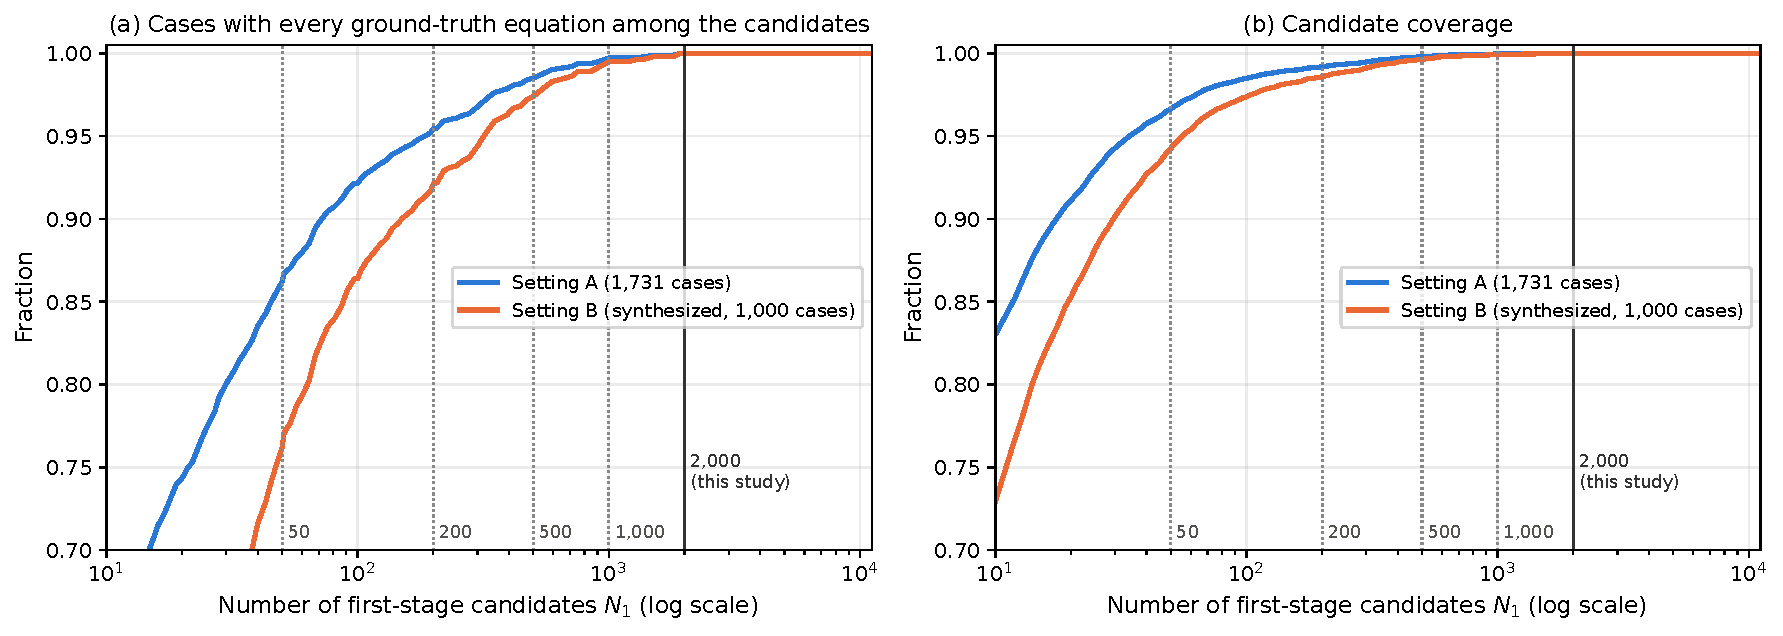
\includegraphics[width=\linewidth]{figures/fig_n1_coverage.pdf}
\caption{Number of first-stage candidates $N_1$ (log scale) and (a) the fraction of cases with
every ground-truth equation among the candidates and (b) the candidate coverage, the fraction of
ground-truth equations among the candidates (first-stage weights $(\WText, \WVar)$). Dotted lines
mark the values of $N_1$ compared in Table~\ref{tab:n1}, and the solid line the $N_1 = \NOne$ of
this study. Every ground-truth equation of every case enters the candidates at
$N_1 = \NOneAllGt$.}
\label{fig:n1}
\end{figure}
